\documentclass[11pt,compress,t,notes=noshow, aspectratio=169, xcolor=table]{beamer}

\usepackage{../../style/lmu-lecture}
% Defines macros and environments
% This file is included in slides and exercises

% Rarely used fontstyle for R packages, used only in 
% - forests/slides-forests-benchmark.tex
% - exercises/single-exercises/methods_l_1.Rnw
% - slides/cart/attic/slides_extra_trees.Rnw
\newcommand{\pkg}[1]{{\fontseries{b}\selectfont #1}}

% Spacing helpers, used often (mostly in exercises for \dlz)
\newcommand{\lz}{\vspace{0.5cm}} % vertical space (used often in slides)
\newcommand{\dlz}{\vspace{1cm}}  % double vertical space (used often in exercises, never in slides)
\newcommand{\oneliner}[1] % Oneliner for important statements, used e.g. in iml, algods
{\begin{block}{}\begin{center}\begin{Large}#1\end{Large}\end{center}\end{block}}

% Don't know if this is used or needed, remove?
% textcolor that works in mathmode
% https://tex.stackexchange.com/a/261480
% Used e.g. in forests/slides-forests-bagging.tex
% [...] \textcolor{blue}{\tfrac{1}{M}\sum^M_{m} [...]
% \makeatletter
% \renewcommand*{\@textcolor}[3]{%
%   \protect\leavevmode
%   \begingroup
%     \color#1{#2}#3%
%   \endgroup
% }
% \makeatother


\title{Interpretable Machine Learning}
% \author{LMU}
%\institute{\href{https://compstat-lmu.github.io/lecture_iml/}{compstat-lmu.github.io/lecture\_iml}}
\date{}

\begin{document}

\newcommand{\titlefigure}{figure/iml_level_1}
\newcommand{\learninggoals}{
\item[] \hspace {-2.5em}  Understand Interpretation Goals: 
\item Global insights (discovery)
\item Improve model (debug and audit)
\item Understand and control individual predictions
\item Justification and fairness}

\lecturechapter{Interpretation Goals}
\lecture{Interpretable Machine Learning}

% \begin{frame}{Why Interpretability?}
% % 		\begin{itemize}
% % 			\item Machine learning (ML) has a huge potential to aid the decision-making process in various  applications.
% % 			\pause
% % 			\smallskip
% % 			\item ML models often are intransparent black boxes, e.g., XGBoost, RBF SVM, or NNs.
% % 			\begin{itemize}
% % 				\item[$\rightarrow$] too complex to be understood by humans.
% % 			\end{itemize}
% % 			\smallskip
% % 			\item A lack in explanations diminishes trust in the model and creates barriers for adoption, especially in areas with critical decision-making consequences, e.g., medicine.
% % 			\smallskip
% % 			\item Such disciplines often rely on traditional models,\\ e.g., linear models, with less predictive performance.
% % 			\smallskip
% % 			\item Interpretable machine learning (IML) aims to bridge the gap between interpretability and predictive performance.
% % 		\end{itemize}
% \bigskip
%     \begin{columns}[T, totalwidth=\textwidth]
%     \begin{column}{0.8\textwidth}
% 		\begin{itemize}
% 			\item ML: huge potential to aid decision-making process due to its predictive performance
% 			%\pause
% 			%\smallskip
% 			\only<2->{\item ML models are often black boxes, e.g., XGBoost, RBF SVM or DNNs
% 			\begin{itemize}
% 				\item[$\leadsto$] too complex to be understood by humans
% 			\end{itemize}}
% 			%\pause
% 			%\smallskip
% 			\only<3->{\item Lack of explanation
% 			\begin{enumerate}
% 				\item hurts trust
% 				\item creates barriers
% 			\end{enumerate}}
% 			\only<4->{\item[$\leadsto$] Harder to adapt for critical areas with decisions affecting human life}
% 			\item<5>[\,$\leadsto$] Many disciplines with required trust rely on traditional models,\\ e.g., linear models, with less predictive performance
% 		\end{itemize}
% 	\end{column}
% 	\begin{column}{0.2\textwidth}  %%<--- here
%         \only<2->{\includegraphics[width=0.9\textwidth]{figure/nn_model.png}}
%         \only<2->{\includegraphics[width=0.9\textwidth]{figure/nn_landscape.png}
%         \centering \citebutton{Liu 2021}{https://davideliu.com/2021/12/12/visualizing-loss-landscape-of-gail/}}
%     \end{column}
%     \end{columns}
%     % \bigskip
%     % \begin{columns}[T, totalwidth=\textwidth]
%     %     \begin{column}{0.5\textwidth}
%     %     \begin{itemize}
%     %         \only<5>{\item[$\leadsto$] Harder to adapt for critical areas with decisions affecting human life}
%     %         \item<5>[\,$\leadsto$] Many disciplines with required trust rely on traditional models,\\ e.g., linear models, with less predictive performance
%     %     \end{itemize}
%     %     \end{column}
% 	   % \begin{column}{0.5\textwidth} 
% 	   %     \only<5>{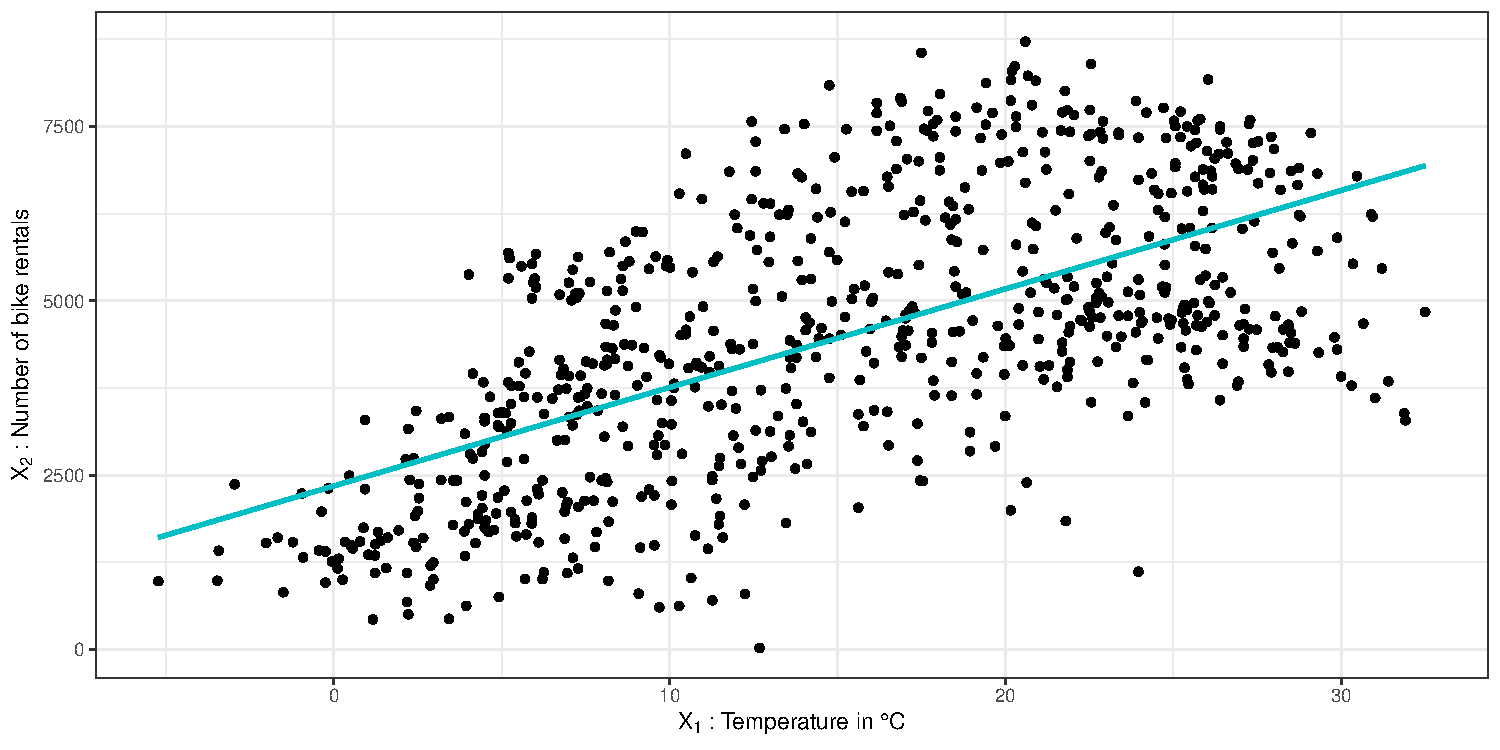
\includegraphics[width=\textwidth]{figure/intro_lm_bike.pdf}}
% 	   % \end{column}
%     %     \end{columns}
% \end{frame}
	
	
% \begin{frame}{Interpretability in High-stakes Decisions}

% Examples of critical areas where decisions based on ML models can affect human life 
%     % \begin{itemize}
%     %     \item Credit scoring and insurance applications
%     %     \citebutton{Society of Actuaries}{https://www.soa.org/resources/research-reports/2021/interpretable-machine-learning}
%     % \end{itemize}
%     \begin{columns}[T, totalwidth=\textwidth]
%     \begin{column}{0.55\textwidth}
% 		\begin{itemize}
% 		\item Credit scoring and insurance applications
%         \citebutton{Society of Actuaries}{https://www.soa.org/resources/research-reports/2021/interpretable-machine-learning}
%         \begin{itemize}
%             \item Providing reasons for not granting a loan
%             \item Fraud detection in insurance claims
%         \end{itemize}
%         \item<2-> Medical applications
%         \begin{itemize}
%             \item Identification of diseases
%             \item Chance of recovering
%             \item Recommendations of treatments
%         \end{itemize}
%         \item<2-> \ldots
%     \end{itemize}
%     \end{column}
% 	\begin{column}{0.45\textwidth}
%         \includegraphics<1->[page=1, width=\textwidth, trim = 0 250 0 0, clip]{figure/counterfactual.pdf}
%         \medskip
% 	    \only<2->{\includegraphics[width=\textwidth]{figure/medicine.png}
% 	    \centering \citebutton{Miliard (2020)}{https://www.healthcareitnews.com/news/new-ai-diagnostic-tool-knows-when-defer-human-mit-researchers-say}}
% 	\end{column}
%     \end{columns}
% \end{frame}


% \begin{frame}{Need for interpretability in High-stakes Decisions}

%     Need for interpretability also becoming increasingly important from a legal perspective
    
%     \begin{itemize}
%     \item General Data Protection Regulation (GDPR) requires for some applications that models have to be explainable \citebutton{Goodman \& Flaxman (2017)}{https://doi.org/10.1609/aimag.v38i3.2741}\\
%     $\leadsto$ \textit{EU Regulations on Algorithmic Decision-Making and a ``Right to Explanation''} 
    
%     \item \textit{Ethics guidelines for trustworthy AI}
%     \citebutton{European Commission (2019)}{https://doi.org/10.2759/346720}

%     \end{itemize}
%     \medskip
    
%     \centering\includegraphics[width=0.7\textwidth]{figure/compass_black_white.PNG}
%     % source https://www.propublica.org/article/how-we-analyzed-the-compas-recidivism-algorithm
% \end{frame}


% 	%-----------------------------------------------------------------------------------------------------------------------------

% \begin{frame}{Brief History of Interpretability}
% 	\begin{columns}[T, totalwidth=\textwidth]
% 	\begin{column}{0.75\textwidth}
% 	    \begin{itemize}
% 			\item 18th and 19th century: \\linear regression models (Gauss, Legendre, Quetelet)
% 			\medskip
% 			\item<2-> 1940s:\\ emergence of sensitivity analysis (SA)
% 			\medskip
% 			\item<3-> Middle of 20th century:\\ Rule-based ML, incl. decision rules and decision trees
% 			\medskip
% 			\item<4-> 2001:\\ built-in feature importance measure of random forests
% 			\medskip
% 			\item<5-> >2010: \\Explainable AI (XAI) for deep learning
% 			\medskip
% 			\item<6> >2015: \\IML as an independent field of research
% 		\end{itemize}
% 	\end{column}
% 	\begin{column}{0.25\textwidth}
% 	    \includegraphics[width=0.8\textwidth]{figure/Carl_Friedrich_Gauss_1828.jpg}
%         \centering \citebutton{Carl Friedrich Gauss}{https://commons.wikimedia.org/w/index.php?curid=2404149}
%         \centering \citebutton{Wikipedia}{https://en.wikipedia.org/wiki/Carl_Friedrich_Gauss}
%         \bigskip\\
%         \only<3->{\includegraphics[width=0.9\textwidth]{figure/Random_Forest.png}}
%         % https://docs.google.com/presentation/d/15HjwMHdTtZ9N0cniUPsiztRSRg1UDY3Y5M8tXsaqt2I/edit?usp=sharing
% 	\end{column}
% 	\end{columns}
% \end{frame}

	%-----------------------------------------------------------------------------------------------------------------------------
% \begin{frame}{When do we need interpretability?}
% \begin{columns}[T, totalwidth=\textwidth]
% \begin{column}{0.6\textwidth}
% %  \begin{itemize}
% %   \item Debugging machine learning models
% %   \item Increasing trust in models
% %   \item Analyzing newly developed systems with unknown consequences
% %   \item Decisions about humans
% %   \item Models using proxies instead of causal inputs, e.g. predicting flu outbreaks from google searches.
% %   \item When loss function does not cover constraints like fairness (e.g. credit score) or need for insights (e.g. science).
% % \end{itemize}
% \begin{itemize}
%   \item To \textbf{Discover}: Gain insights about data, distribution and model
%   \pause 
%   \item To \textbf{Debug, audit and improve}: Insights help to identify flaws (in data or model), which can be corrected (debug and audit)\\
%   $\leadsto$ Global perspective
%   \pause
%   \item To \textbf{explain individual decisions}: Explaining individual decisions can prevent unwanted actions based on the model\\
%   $\leadsto$ Local perspective
%   \pause 
%   \item To \textbf{Justify}: Investigate if and why biased, unexpected or discriminatory predictions were made, or improve/reject the model\\
%   $\leadsto$ Fairness perspective

% \end{itemize}
% \end{column}
% \begin{column}{0.4\textwidth}  %%<--- here
%  %\vspace{0.5cm}
% %  \begin{center}
% %  \begin{figure}
%   \includegraphics[width=0.9\textwidth]{figure/explain-to}
%   \centering \citebutton{Adadi and Berrada 2018}{https://doi.org/10.1109/ACCESS.2018.2870052}
% %  \end{figure}
% %  \end{center}
% \end{column}
% \end{columns}
%      %\lz
%     %\footnote[frame]{Doshi-Velez, F., \& Kim, B. (2017). Towards A Rigorous Science of Interpretable Machine Learning. arXiv: 1702.08608.}
%     %\footnote[frame]{A. Adadi and M. Berrada, "Peeking Inside the Black-Box: A Survey on Explainable Artificial Intelligence (XAI)," in IEEE Access, vol. 6, pp. 52138-52160, 2018.}
% \end{frame}

\begin{frame}{Potential Interpretation Goals}

% \begin{columns}[T, totalwidth=\textwidth]
  %   \begin{column}{0.8\textwidth}
		\begin{center}
            \def\firstcircle{(90:1cm) circle (2.5cm)}
            \def\secondcircle{(210:2.5cm) circle (2.5cm)}
            \def\thirdcircle{(330:2.5cm) circle (2.5cm)}
            \def\fourthcircle{(90:-3.5cm) circle (2.5cm)}
            \resizebox{6.5cm}{6.5cm}{
            \begin{tikzpicture}
                \begin{scope}[ fill opacity=0.5]
                    \fill[red] \firstcircle;
                    \fill[green] \secondcircle;
                    \fill[blue] \thirdcircle;
                    \fill[cyan] \fourthcircle;
                \end{scope}
                \draw \firstcircle node[text=black,above, text width=2cm, align=center] {To discover and gain global insights};
                \draw \secondcircle node [text=black, left, text width=2cm, align=center] {To improve, debug and audit models};
                \draw \thirdcircle node [text=black,right, text width=2cm, align=center] {To understand and control individual predictions};
                \draw \fourthcircle node [text=black,below, text width=2cm, align=center]{For justification and fairness purposes};
            \end{tikzpicture}}
        \end{center}
 %    \end{column}
	% \begin{column}{0.2\textwidth}
 %        \centering \citebutton{Miliard (2020)}{https://www.healthcareitnews.com/news/new-ai-diagnostic-tool-knows-when-defer-human-mit-
	% \end{column}
 %    \end{columns}

\footnote[frame]{A related presentation can be found in \citebutton{Adadi and Berrada 2018}{https://doi.org/10.1109/ACCESS.2018.2870052}.}

\end{frame}



% \begin{frame}{Why is Interpretability Important?}

% 	\begin{itemize}
% 	    \item Machine learning is (mostly) about discovering patterns in data.
% 	    \medskip
% 	    \item Unfortunately, it is not guaranteed that ML will identify the correct patterns.

% 	    \medskip
% 	    \item We humans might not be able to discover patterns ML models discovered.
% 	    \begin{itemize}
% 	        \item Good for science or to get new insights.
% 	        \item Bad in applications where unexpected behavior is not desired.
% 	    \end{itemize}
% 	    \medskip

% 	    \item \alert{How can you check whether the model is correct in its inference?}
% 	\end{itemize}

% \end{frame}

\begin{frame}{Discover and gain global insights}
$\leadsto$ Gain insights about data, model, and underlying data-generating process \\
\medskip
\textbf{Example:} Bike Sharing Dataset (predict number of bike rentals per day) \\
\textit{Exemplary question:} Which feature influences model performance and how much?
\begin{center}
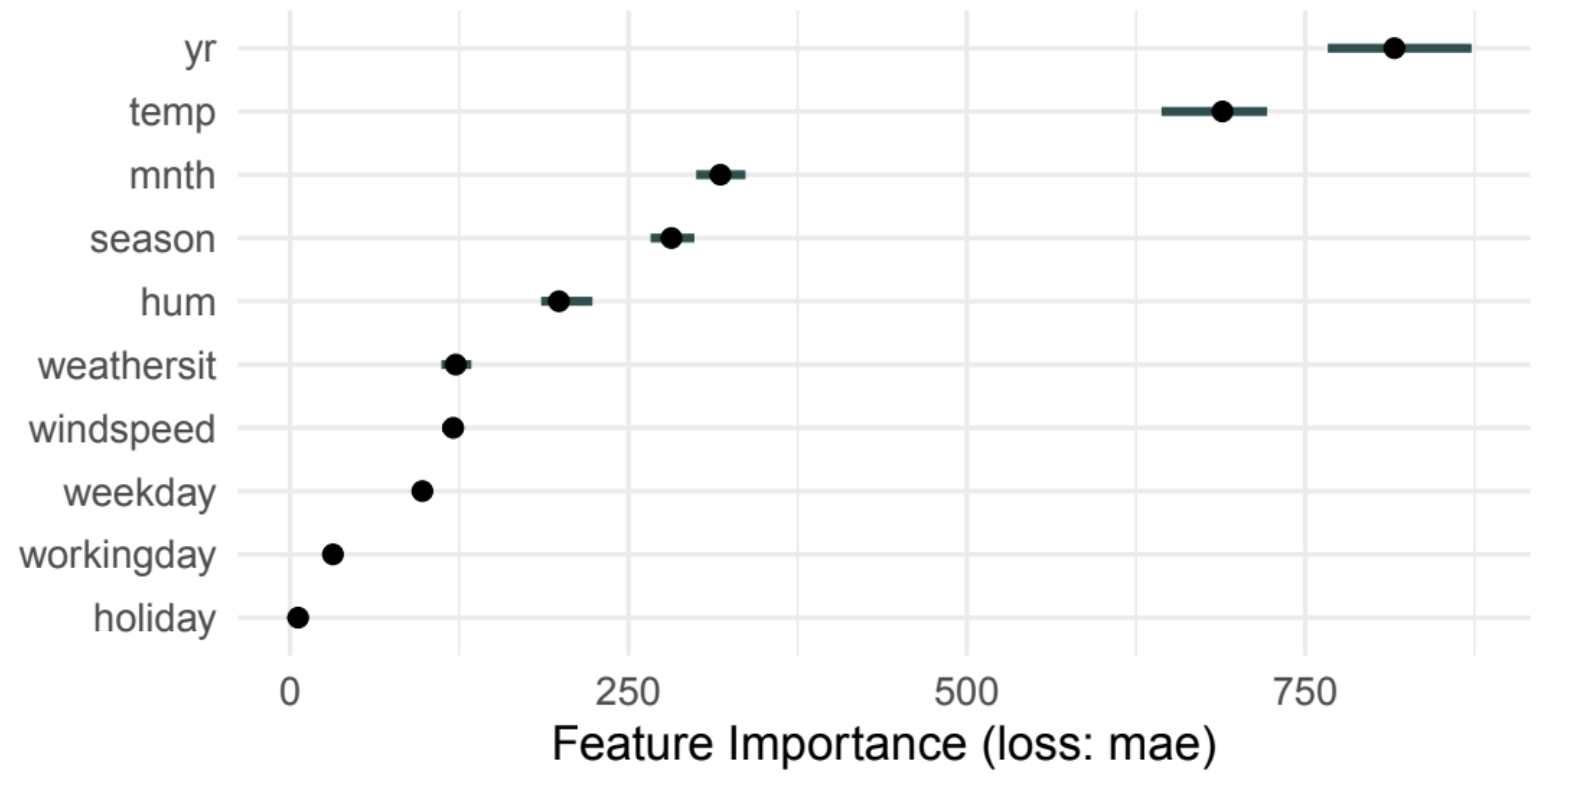
\includegraphics[width=0.8\textwidth]{figure/bike-sharing02.png}
\end{center}

%\textbf{Interpretation:}

\begin{itemize}
    \item Year (\code{yr}) and Temperature (temp) most important features
    \item Holiday (\code{holiday}) less important (Can we drop it?)
\end{itemize}

\end{frame}

% \begin{frame}{Example (Improve, debug and audit models): Clever Hans \citebutton{Lapuschkin et al. 2019}{https://www.nature.com/articles/s41467-019-08987-4} }

% 	\centering
% 	\begin{columns}[T, totalwidth=\textwidth]
% 	\begin{column}{0.6\textwidth}
% 	\includegraphics<1>[width=\textwidth]{figure/horse_without_label.PNG}
% 	\includegraphics<2>[width=\textwidth]{figure/horse_with_label.PNG}
% 	\includegraphics<3>[width=\textwidth]{figure/horse_map_with_label.PNG}
% 	\includegraphics<4>[width=\textwidth]{figure/horse_map_without_label.PNG}
% 	\end{column}
% 	\begin{column}{0.4\textwidth}

% 	\begin{itemize}
% 	    \item Horse with claimed math skills
% 	    \item Answered questions correctly by hoof tapping or head shaking
% 	    \item Correct answers were traced to involuntary cues from human's body language $\Rightarrow$ no math skills %asking person
% 	    %(e.g., tense attitude)
% 	    \item<2-> Image classification: \\
% 	    source tag present \\
% 	    \onslide<3->{$\Rightarrow$ classified as horse}
% 	    \item<4-> no source tag \\ $\Rightarrow$ not classified as horse
% 	\end{itemize}

% 	\end{column}
% 	\end{columns}
% \end{frame}

\begin{frame}{Improve, debug and audit models}
$\leadsto$ Insights help to identify flaws (in data or model), which can be corrected \\
\medskip
\textbf{Example:} Neural Net Tank \citebutton{gwern.net}{https://www.gwern.net/Tanks} \\
	\centering
	\begin{columns}[T, totalwidth = \textwidth]
	\begin{column}{0.44\textwidth}
	\centering
	% pictures from pixabay
	\only<1>{\includegraphics[width=\textwidth]{figure/tank.jpg}}
	\only<2>{
        \begin{figure}
            \centering
            \begin{tabular}{@{}c@{}}
                \includegraphics[width=0.65\textwidth]{figure/tank.jpg}
            \end{tabular}

            \begin{tabular}{@{}c@{}}
        	    \includegraphics[width=0.65\textwidth]{figure/landscape.jpg}
            \end{tabular}
        \end{figure}
    }
    \only<3>{
            \includegraphics[width=0.48\textwidth]{figure/tank.jpg}
            \includegraphics[width=0.48\textwidth]{figure/tank_green.jpg}
	        \includegraphics[width=0.48\textwidth]{figure/landscape.jpg}
	        \includegraphics[width=0.48\textwidth]{figure/landscape_green.jpg}}
	\end{column}
	\begin{column}{0.56\textwidth}
    \hspace{0.1cm} Cautionary tale (never actually happened):
	\begin{itemize}
	    \item Train a neural network to detect tanks
        \item Good fit on training data
        \item Application outside training data: failure
        \item<2-> Reasons vary depending on input\\
        $\leadsto$ NN based decision on irrelevant pixels
        \item<3-> E.g. model detects weather based on sky:\\
        $\leadsto$ All photos with tanks show cloudy sky\\
        $\leadsto$ Photos without tanks show sunny sky
	\end{itemize}

	\end{column}
	\end{columns}

\end{frame}

\begin{frame}{Improve, debug and audit models}
$\leadsto$ Insights help to identify flaws (in data or model), which can be corrected \\[2ex]
	\centering
    Comment on tank example: 
    \begin{quote}
        ''We made exactly the same mistake in one of my projects on insect recognition. We photographed 54 classes of insects. Specimens had been collected, identified, and placed in vials. Vials were placed in boxes sorted by class. I hired student workers to photograph the specimens.\\[0.5ex]
        Naturally they \textbf{did this one box at a time; hence, one class at a time.} Photos were taken in alcohol. \textbf{Bubbles would form in the alcohol. Different bubbles on different days.} The learned classifier was surprisingly good. But a \textbf{saliency map revealed that it was reading the bubble patterns} and ignoring the specimens.\\[0.5ex]
        I was so embarrassed that I had made the oldest mistake in the book (even if it was apocryphal). Unbelievable.
        Lesson: always randomize even if you don’t know what you are controlling for!''
    \end{quote}
    \citebutton{Thomas G. Dietterich}{https://x.com/tdietterich/status/1154839042623594496}
 \end{frame}

\begin{frame}{Debug and Audit}
    \begin{itemize}
        %\item etwas mehr die "technische" perspektive bringen und ein paar zeilen hintergrund was debuggiung ist, warum es schon immer schwierrig war und mit ML die hölle wird. ein porgramm schreibt ein program
        \item Nearly all computer programs have bugs
        \begin{itemize}
            \item[$\leadsto$] Minimizing such bugs extremely relevant
        \end{itemize}
        \item Process with multiple steps to locate, understand and solve a problem
        \begin{itemize}
            \item[$\leadsto$] Classical debugging
        \end{itemize}
        \item \textbf{In ML} we have a program (learner) writing another program (model)
        \item How to debug or audit programs which contain ML models? 
        \item Based on a single cross-val score?
            \item[$\leadsto$] Being able to interpret your model will always be helpful -- if possible!
            % \item[$\leadsto$] Simplify as far as possible
            % \item[$\leadsto$] Verify the mathematics
            % \item[$\leadsto$] Make the code more complex step by step
    \end{itemize}
\end{frame}

% \begin{frame}{Clever Hans \citebutton{Lapuschkin et al. 2019}{https://www.nature.com/articles/s41467-019-08987-4}}

% 	\centering
% 	\includegraphics[width=0.6\textwidth]{figure/boats_maps.PNG}

% \end{frame}

\begin{frame}{Understand \& control individual predictions}
    $\leadsto$ Explaining individual decisions can prevent unwanted actions based on the model \\
    \medskip
    \textbf{Example:} Credit Risk Application\\
    $\textbf{x}$: customer and credit information; $y$: grant or reject credit
	
	\only<1>{\begin{center}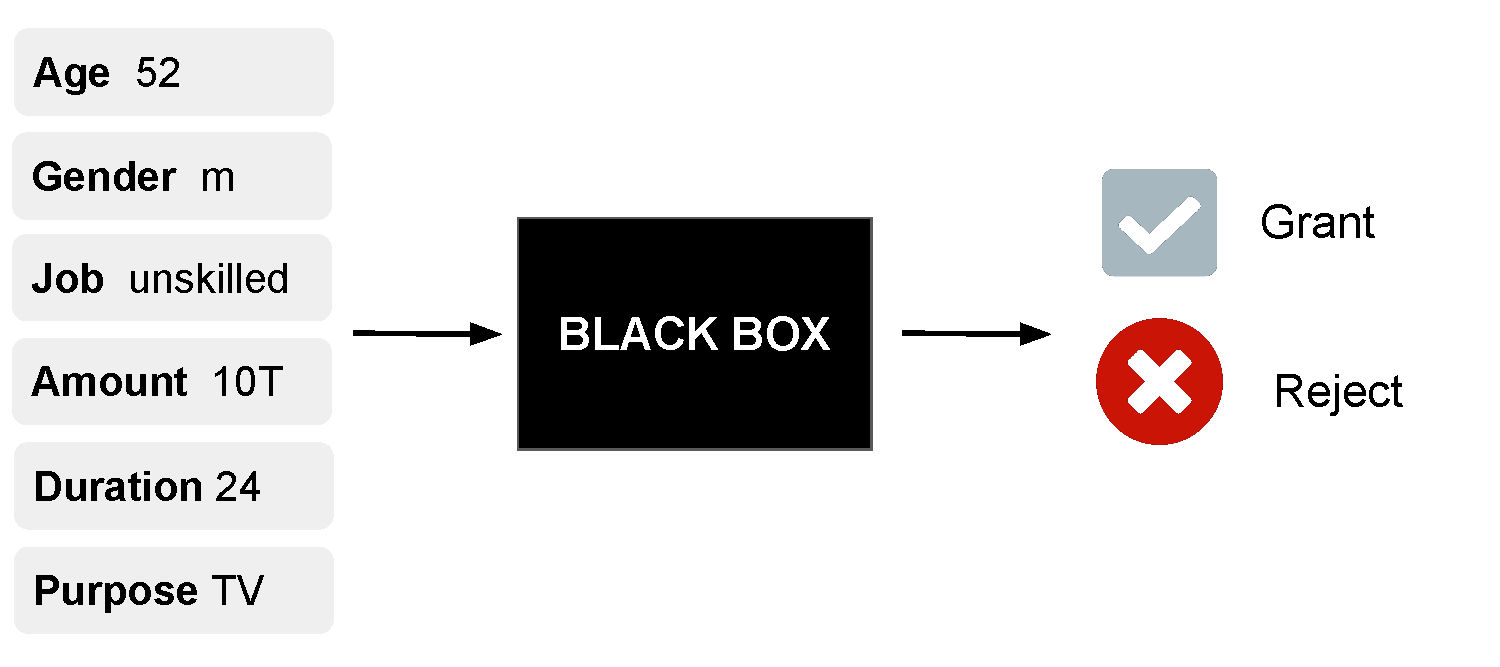
\includegraphics[width=0.6\linewidth, page=1]{figure/counterfactuals_credit.pdf} \end{center}

	Questions:}
	\begin{itemize}
		\item Why was the credit rejected?
		\item Is it a fair decision?
		\item \textbf{How should $\xv$ be changed so that the credit is accepted?}
	\end{itemize}
	
	%Counterfactual Explanations provide answers in the form of "What-If"-scenarios.
	\only<2>{\begin{center}\includegraphics[width=0.6\linewidth, page=2]{figure/counterfactuals_credit.pdf} \end{center}

	``If the person was more skilled and the credit amount had been reduced to \$8.000,\\ the credit would have been granted."} 
\end{frame}

%%%

\begin{frame}{Justification and fairness}
    $\leadsto$ Investigate if and why biased, unexpected or discriminatory predictions were made \\
    \bigskip
    \textbf{Example:} COMPAS
    \smallskip
    \begin{itemize}
        \item COMPAS: Correctional Offender Management Profiling for Alternative Sanctions
    \item Commercial tool used in courts to assess a defendant’s risk of re-offending

    \item Predicts \textbf{recidivism risk}:
    \begin{itemize}
        \item Likelihood of an individual with a past offense is arrested again
        \item Features: race, gender, age, number of prior prison sentences, ...
        \item Output: COMPAS score from 1 (low risk) to 10 (high risk) risk of recidivism
    \end{itemize}
    \item Based on a questionnaire completed by the defendant
    \end{itemize}

\end{frame}

\begin{frame}{Justification and fairness: COMPAS~\citebutton{Larson et al. 2016}{https://www.propublica.org/article/how-we-analyzed-the-compas-recidivism-algorithm}}
    $\leadsto$ Investigate if and why biased, unexpected or discriminatory predictions were made \\
    \medskip
    Descriptive data analysis of the target (COMPAS score) by a feature encoding race: 

    \medskip
    \centering
    
    \hspace{20pt} Caucasian \hspace{100pt}
 African American
    \includegraphics[trim=0 20 0 50, width=0.95\textwidth, clip]{figure/compass_black_white.PNG}
    % source https://www.propublica.org/article/how-we-analyzed-the-compas-recidivism-algorithm

    COMPAS score: 1 (low risk) to 10 (high risk)

    \medskip
    \raggedright
	$\leadsto$ Model skewed towards low risk for Caucasians
	
	$\leadsto$ Strong indication that the model is discriminating against African American
	
	$\leadsto$ Use IML to investigate if and how much the model uses the defendant's race
\end{frame}

\begin{frame}{Justification and fairness: COMPAS \citebutton{Alvarez-Melis and Jaakkola 2018}{https://arxiv.org/pdf/1806.08049.pdf}}

    $\leadsto$ Investigate if and why biased, unexpected or discriminatory predictions were made 

\medskip

    IML: Analyze how strongly a feature influences an individual prediction (e.g., LIME):

    \medskip
    \centering
    
       \begin{columns}[T, totalwidth=\textwidth]
        \begin{column}{0.5\textwidth}
            
    \includegraphics[trim=695 50 5 0, width=0.95\textwidth, clip]{figure/COMPAS_shap_lime_example.png}
        \end{column}
        \begin{column}{0.5\textwidth}
        \begin{itemize}
            \item Pick a defendant
            \item LIME quantifies a feature's impact on the defendant's COMPAS score
            \item \texttt{African\_American} has a large positive weight on COMPAS score
            \item Occurs for many individuals, see
            \citebutton{XAI Stories}{https://pbiecek.github.io/xai_stories/story-compas.html\#model-specific}
            $\leadsto$ Suggests racial bias
        \end{itemize}
        
        \end{column}
    \end{columns}
\end{frame}





% \begin{frame}{Motivation - Adversarial Examples \citebutton{Goodfellow et al. 2016}{https://arxiv.org/pdf/1412.6572.pdf}}

%     \begin{center}
%     \includegraphics[width=0.7\textwidth]{figure/panda-airplane.pdf}
%     \end{center}
% 	\bigskip

% 	$\rightarrow$ ML Models might not capture human-like understanding
% \end{frame}


% \begin{frame}{Adversarial Noise \citebutton{Goodfellow et al. 2016}{https://arxiv.org/pdf/1412.6572.pdf}}
%     \begin{center}
%     \includegraphics[width=0.65\textwidth]{figure/adv-noise.pdf}
%     % https://arxiv.org/pdf/1412.6572.pdf
% 	\end{center}
% 	\normalsize
% 	%\bigskip
% 	$\rightarrow$\textbf{Adversarial Noise:} Noise not visible to \textbf{humans} but results in incorrect classification results
% \end{frame}

% \begin{frame}[c]{Adversarial Examples~\citebutton{Goodfellow et al. 2016}{https://arxiv.org/pdf/1412.6572.pdf}}
    
%     \centering
%     \includegraphics[width=0.7\textwidth]{figure/adv-noise-2.pdf}
	
% \end{frame}

% \begin{frame}{Performance vs. Interpretability}
%     \centering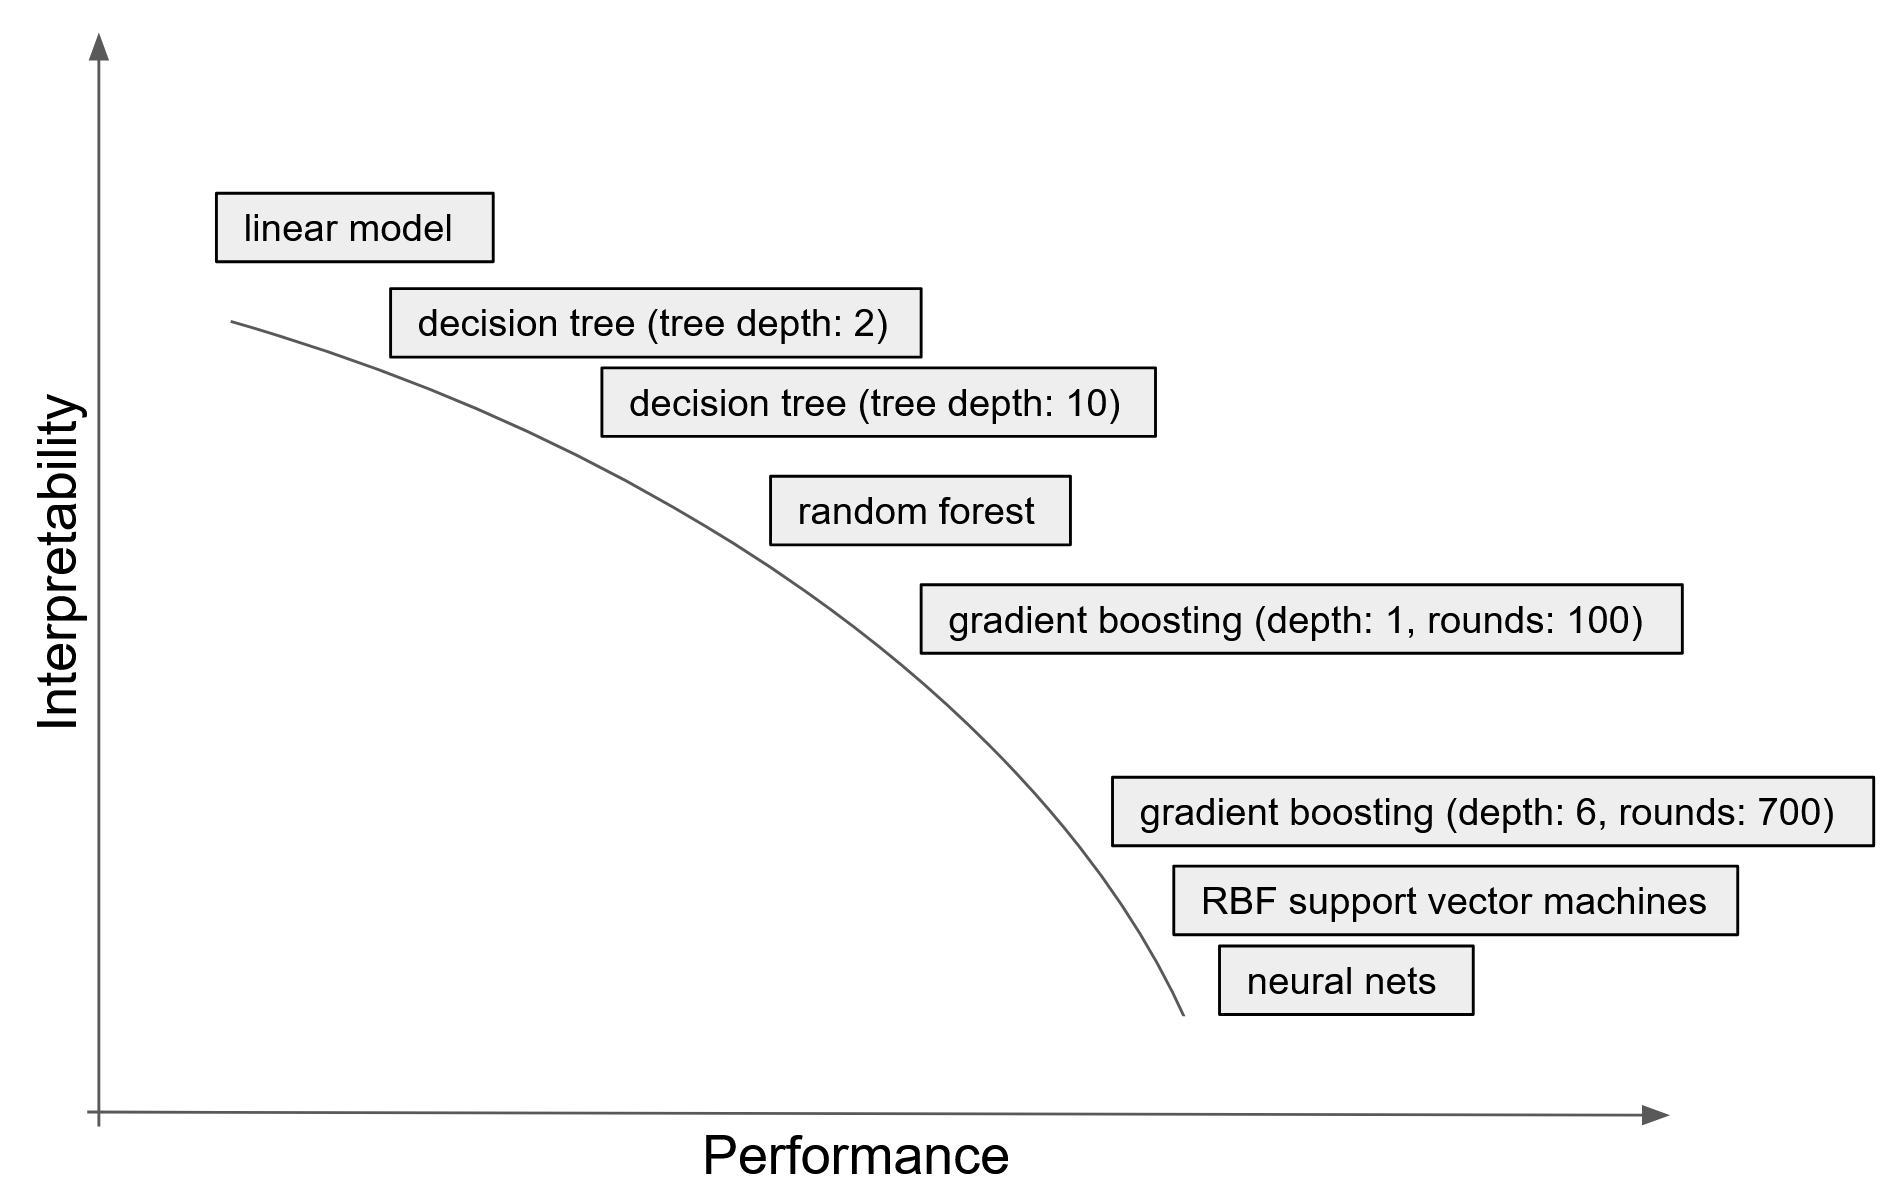
\includegraphics[width=0.7\textwidth]{figure/performance_vs_interpretability.png}
%     % Quelle: https://docs.google.com/presentation/d/12ZPrTjBKEUT-7drdyUJCQGK0oHVDtYIVd2_6byE62f0/edit?usp=sharing
%     %\centering \citebutton{Scott Fortmann-Roe (2012)}{http://scott.fortmann-roe.com/docs/BiasVariance.html}
% \end{frame}

\endlecture
\end{document}
